% !TEX root = ../main.tex
This section will reflect and discuss the reached solution, based upon tests and the results therefrom. It will elaborate on the parts of the problems, which was not solved. And finally reflect upon the project as a whole.

\subsection{Not Solved}
We wanted to create a web client, which should include a suite of administrative tools, for the municipality workers to use, to select issues to solve. In this web client, we would have solved the prioritization problem. But as we have not created this web client, as we deemed it out of the scope of the course, which focuses on mobile sensing.

Although it has not been implemented, we have made the architecture of our server application ready to serve a web client, and we believe that it would not be of great risk to implement such a client.
~\\

The lacking incentive for using the platform, has not been implemented in this prototype application, but it have been addressed, with the three solution suggestions from section X (ref 3). We have analyzed the three solutions and found both pros and cons for all implementations, and found that the lottery solution might promote cheating for personal materialistic gain, and would therefore not pursue that solution. And we found that the charity solution, was a good idea, as it could engage users, but it requires external investors in order to become a successful solution. Therefore, we find that the leaderboard solution is the easiest solution, as it do not require any external investors, and does not promote cheating by materialistic gain, but it might not be the most engaging gamification element. We therefore suggest that a combination of the three would be a great solution.
~\\

The reports in the current Giv et Tip application, has categories and images, both of which have not been implemented in this prototype, as it did not add any value to the problem domains. Although the categories could be used for weighing the prioritizations in the web client, so that more demanding categories would be weighed higher that less demanding categories.

\subsection{Project Reflection}
We have tried to utilize an agile approach to the development of the application, where we started by identifying the use cases, and assigned them to weekly sprints, and used a kanban system on GitHub, to keep track of the development progress. This system has worked out well for us, although we moved away from the weekly sprints, and just implemented the features, as we had time for it.
~\\

The project pitch at Odense Castle went well, this project won the “Giv et Tip” project category, and one of the judges, a developer from sweco, mentioned that we had a useful focus, with the crowdsourcing of verification.
~\\
The teamwork within the team, has worked out great, there has been great information and knowledge sharing throughout the process of this project.

\subsection{Known Issues}

\begin{description}
\item [Location permissions:] There is an issue with the location service, the first time the application is started, which renders the location service useless, as it never updates, unless the application is force-stopped, through the android application settings menu. This issue is caused by the lacking confirmation whether GPS is enabled on the first startup of the application. It could probably be fixed by waiting to start the location service until it is known that GPS is enabled.
\item [Shared preferences as storage:] The prototype makes excessive use of the shared preferences as data persistence. This is not optimal, and it would be much better to use SQLite, which is already included in android, for this purpose.
\item [Disabled location services:] There is another issue, which renders the location service useless. If the user disables the location services, in the android settings menu, the application will not prompt the user to re-enable it, when in the application is in focus, in order to make it usable again
\item [Download and storage of reports:] the background service is responsible for keeping report data up to date, by downloading report coordinates over time. It is currently configured to do this on a two hour interval. It would be nice to have some kind of manual update, which would offer users the option to force update the reports. Furthermore, these report coordinates is the only stored data about the reports. This means that every time the user needs to be shown report details, the application needs to download data for that report, and it is then thrown away afterwards.
\item [Settings:] the settings menu in the prototype only offers the option to tune the distance threshold to reports before a notification is shown. It could be great if there was some kinds of settings profiles in stead, which could offer e.g. a power saver mode, a  normal mode, and a power hungry mode. These profiles would be easier for an end user to understand the effects of.
\item [Geofences:] The prototype does not utilize the android api geo-fences, for figuring out which reports to calculate the distance to, but instead just calculates the distance to each and every report. This means that the application uses unnecessarily much processing power to calculate distances to reports, which are multiple kilometers away.
\item [Increased precision around already notified reports:] The prototype do not discriminate between new reports and reports it has already notified the user about, when it comes to calculating the distance to the reports. This means that it increases the GPS sensing precision, which is power consuming, for nothing, as the user will not be notified about the report anyways.
\end{description}

\subsection{Discussion}

The project aimed to solve the problem of validation of reports, prioritization of reports, and the lacking incentive of using the platform. All three problems have been addressed in this report, but only the validation problem solution has been implemented.

The validation problem was solved by implementing an infrastructure for crowdsourcing the validation. The infrastructure utilizes a background service, which runs continuously on the phone, and checks if there are nearby reports. The service then notifies the user when within 30 meters of a report. 
This service works as intended, members of the group have been receiving notifications, while not aware that the service ran in the background, about nearby reports. This proves that the service works as intended, as it should not bother the user other than when there are nearby reports.

As for the other two problems, this report has suggested different solutions, which have not been implemented, due to constraints in the scope and time available.

When developing for battery dependent devices like Android it is important to consider the energy efficiency of a solution for the device. A list of QAS and tactics is described in the tactics section \ref{sec:tactics}. In order to validate the tactics Battery Historian has been taken into use \cite{bathist}. This allows for measuring all of the activity on the Android device to be able to determine what is going on while using our app. 

While using battery historian a test was conducted. The device used for testing was a OnePlus 5T running Android 7.1.1. 

Thomas went out for a walk while having the app running in the background. Google Maps Timeline feature was used to track the path Thomas took while testing the application - it is worth mentioning that Google Maps nor any other location tracking service was running while Thomas was walking. \autoref{fig:thomas_walk} shows the path as well as a red circle, which marks the spot where reports were placed in our app.

\begin{figure}[H]
\centering
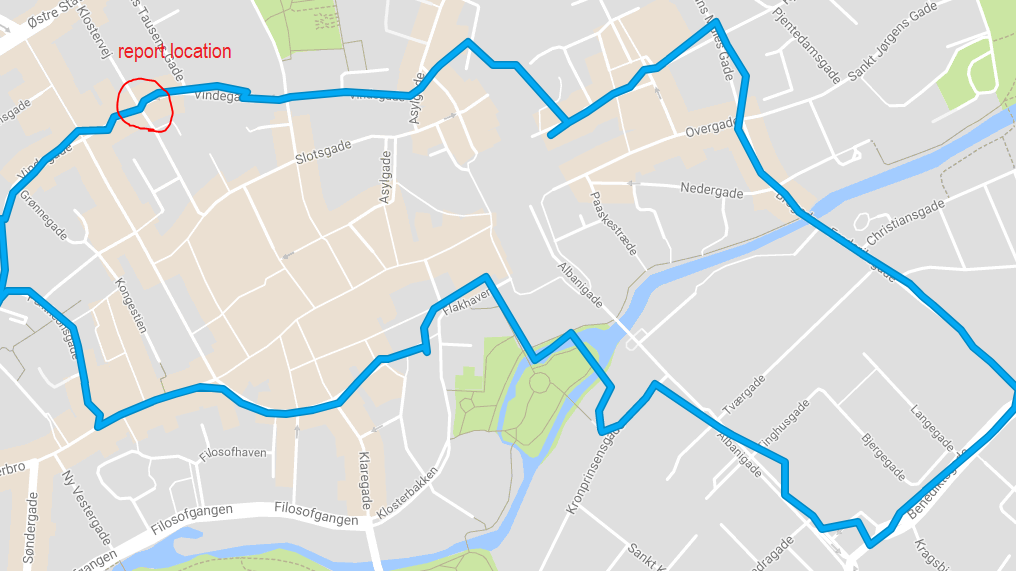
\includegraphics[width=.85\linewidth]{images/thomas_walk}
\caption{Map of the Thomas walk} 
\label{fig:thomas_walk}
\end{figure}


Thomas got a notification as soon as he approached the red circle marked on figure \ref{fig:thomas_walk}. He approached the red circle somewhere around 1:27-1:29 PM according to Google Timeline. It is seen in figure \ref{fig:battery_stats_1} that the GPS is turned on at 1:27:08 PM until 1:30:50 PM. This fits very well into the timestamp provided by Google Timeline - this means that the GPS was turned on around the same time as Thomas was near the report.

\begin{figure}[H]
\centering
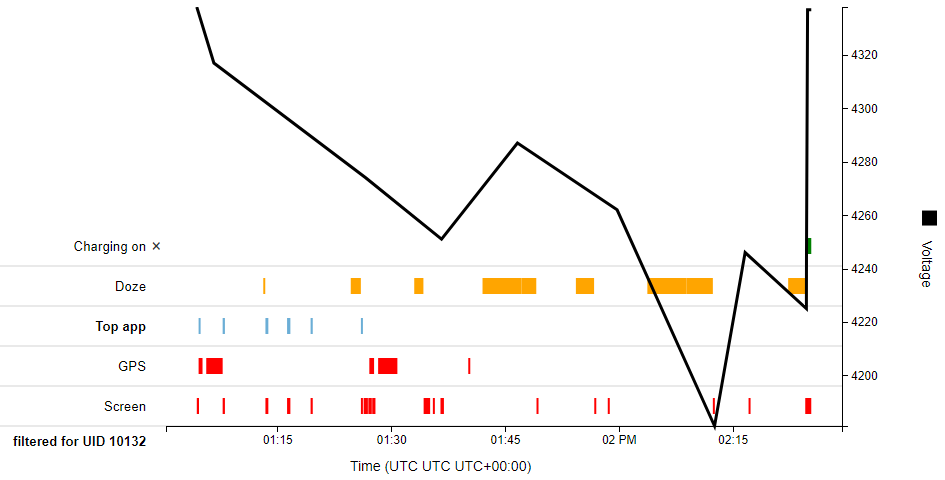
\includegraphics[width=\linewidth]{images/battery_hist}
\caption{Image from Battery Historian.} 
\label{fig:battery_stats_1}
\end{figure}

This confirms that the implementation of dynamic duty cycling works as the location sensor accuracy was changed when Thomas approached and moved away from the report. 

The accumulated discharge throughout the test was 7 percent with a test duration of 1 hour and 20 minutes. The power estimates throughout the test are shown in table \ref{fig:power_estimates}.


\begin{figure}[H]
\centering
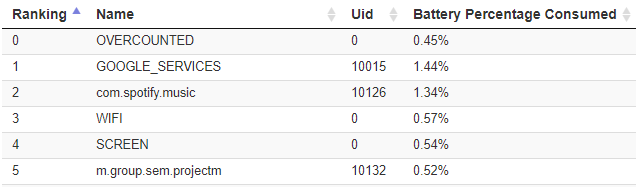
\includegraphics[width=\linewidth]{images/powerestimates}
\caption{Power estimates} 
\label{fig:power_estimates}
\end{figure}

Our solution comes in on a top 5 of the most battery consuming activities with 0.52\% battery consumption. This means that our app is responsible for 7.14\% of the battery consumption throughout the 1 hours and 20 minutes test. Compared to playing music using Spotify for the same duration, the battery consumption of our app is close to just one third of Spotify. 

Increasing the battery consumption by 7.14\% using our application would reduce the battery lifetime - of the device in question - by an estimated 1 hour and 20 minutes. Taking it from a 19 hour battery life to a 17 hour and 50 minutes lifetime. This seems like a fairly acceptable battery consumption considering that the application is relying on very precise GPS positioning. 

Potentially the battery consumption of the application could be reduced by optimizing the background service. Some of the ways to optimze the application are mentioned in the known issues section of the discussion. This includes using the geofencing to reduce activity recognition in the background. Other factors, methods, and tactics can also be investigated further to optimize battery usage.


\vspace{3em}
\hrule
Unsolved tasks has been stated as well as known issues. Project reflection described the agile approach to the project and the discussion section shows the validation and battery consumption test of the application. 